\chapter{Understanding Big-O Through Fibonacci}
\label{ch:big-o-fib}

\section{Why Fibonacci is the Perfect Big-O Lens}
Fibonacci exposes two very different growth stories:
\begin{itemize}
  \item The naive recursive version has \emph{exponential} time, roughly $O(2^n)$.
  \item With memoization (or bottom-up DP), the time drops to \emph{linear}, $O(n)$, with $O(n)$ space.
\end{itemize}
This makes it a great stage to see how algorithm design transforms cost. \,\,\textit{(See Chapters 2--4 for setup and experiments.)} :contentReference[oaicite:0]{index=0}

\section{Deriving the Cost}
\subsection{Naive recursion: $O(2^n)$ time}
Define the cost $T(n)$ of
\[
F(n)=
\begin{cases}
0,& n=0\\
1,& n=1\\
F(n-1)+F(n-2),& n>1
\end{cases}
\]
Each call to $F(n)$ triggers two subcalls (except at base cases). A standard bound is
\[
T(n)=T(n-1)+T(n-2)+O(1) \quad \Rightarrow \quad T(n)=\Theta(\varphi^n),
\]
where $\varphi=\frac{1+\sqrt{5}}{2}\approx1.618$ and $\varphi^n=\Theta(2^n)$.
Intuition: the recursion tree doubles “enough” times that the total work explodes exponentially.

\subsection{Memoization: $O(n)$ time, $O(n)$ space}
Top-down memoization stores previously computed $F(k)$ so each $k\in\{0,\dots,n\}$ is computed once:
\[
T(n)=T(n-1)+O(1), \quad \text{amortized over } n \text{ distinct subproblems} \Rightarrow T(n)=O(n).
\]
Space is $O(n)$ for the table/stack (top-down) or just $O(n)$ array (bottom-up). The iterative two-variable version achieves $O(1)$ extra space.

\section{Visual: Exponential vs Linear}
Figure~\ref{fig:bigocurves} plots $2^n$ against $n$. The lines start friendly, then $2^n$ rockets away like a bottle rocket with a PhD.
\begin{figure}[htbp]
  \centering
  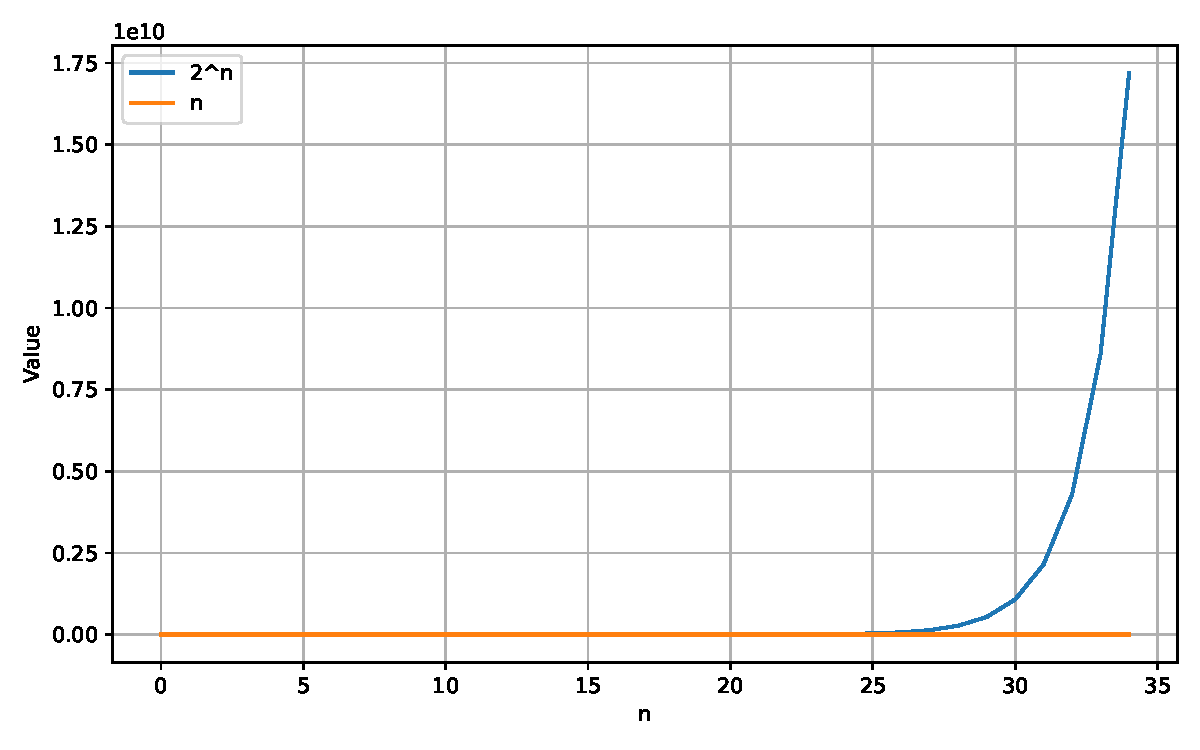
\includegraphics[width=.85\textwidth]{chapters/big_o_curves.pdf}
  \caption{$2^n$ vs $n$ on the same axes (log-scale optional).}
  \label{fig:bigocurves}
\end{figure}

\section{Code: Three Flavors of Fibonacci}
We include three implementations and an experiment harness that writes CSV and plots.

\subsection{Tracker and Implementations}
\lstinputlisting[language=Python,caption={Tracker and Fibonacci variants},label={lst:fib_variants}]{chapters/fib_variants.py}

\subsection{Experiment: timing, counts, and plots}
\lstinputlisting[language=Python,caption={Benchmark and plots for recursive vs memo vs iterative},label={lst:fib_bench}]{chapters/fib_bench.py}

\section{Practical Implications}
\begin{itemize}
  \item \textbf{Naive recursion} demonstrates explosive growth; great teaching tool, terrible production tool beyond modest $n$.
  \item \textbf{Memoization} replaces recomputation with table lookups: a tiny idea with huge consequences.
  \item \textbf{Iterative DP} keeps the wins while minimizing memory; for Fibonacci, two scalars suffice.
\end{itemize}

\section{Optional: Memory Probe (Laptop)}
To show that Big-O is a map (not the terrain), we sample real memory/CPU while the naive version gnaws on the stack. See Listing~\ref{lst:fib_memprobe}.
\lstinputlisting[language=Python,caption={Lightweight memory/CPU probe while running recursion},label={lst:fib_memprobe}]{chapters/fib_memprobe.py}

\section{Student Prompts}
\begin{enumerate}
  \item For which $n$ does naive recursion become impractical on your machine?
  \item Modify memoization to bottom-up; compare peak memory with \texttt{tracemalloc}.
  \item Explain why memoization changes the recursion tree’s shape and total nodes visited.
\end{enumerate}

